\section{Trajektorienplanung}
\label{sec:trajektorienplanung}
Das Auto hat vorne sowie hinten jeweils zwei R\"ader, die durch einen Elektromotor ansteuerbar sind. Die Lenkung der Vorderachse ist durch einen Servomotor realisiert. Das Fahrzeug ist vorne und an den Seiten mit Ultraschallsensoren zur Abstandmessung ausgestattet und besitzt eine nach vorne ausgerichtete Kinect2 Kamera, die sowohl Farb- als auch Tiefenbild liefert. F\"ur die Bestimmung der Orientierung des Fahrzeugs sind verschiedene Sensoren verbaut. \\
Um einen Rundkurs mit oder ohne Hindernissen zu bew\"altigen, muss man die gegebenen Werkzeuge nutzen und entsprechend kombinieren um das Ziel zu erreichen. Die beiden Ans\"atzen \"uber einen PD-Abstandregler (vergleiche Abschnitt \ref{subsec:02PDregler}) und \"uber eine Trajektorienplanung (vergleiche Abschnitt \ref{subsec:02implementierung}) werden im Folgenden vorgestellt.

\subsection{Modellbildung}
\label{subsec:02modellbildung}
Um eine Beziehung zwischen physikalischer Gr\"o\ss{}e f\"ur Geschwindigkeit und Lenkwinkel und der entsprechenden Stellgr\"o\ss{}e zu herzustellen, wird jeweils ein Modell ben\"otigt.
\paragraph{Geschwindigkeitsmodell} %TODO set math envirment
Die Daten aus Abbildung \ref{fig:velocity_profile} wurden bei einer Messfahrt mit Hilfe eines rosbag aufgezeichnet und im Anschluss mit dem Tool plotjuggler ausgewertet. Dazu wurde das Fahrzeug mit Geschwindigkeitsstellgr\"o\ss{}en im Intervall von -500 bis 1000 angesteuert und die jeweilige Geschwindigkeit aus der Odometrie ausgelesen. Auff\"allig ist der Sprung am Achsenursprung, der dadurch entsteht, dass das Fahrzeug eine bestimmte Stellgr\"o\ss{}e ben\"otig, um seine Tr\"agheit zu \"uberwinden.
Die gemessenen Daten lassen sich durch eine Gerade approximieren.

%%Akku
\begin{figure}[h] %TODO replace image
\centering
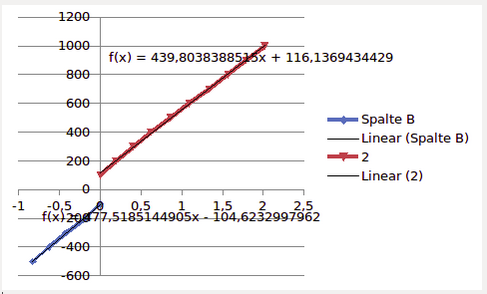
\includegraphics[width=0.7\linewidth]{pics/velocity_profile}
\caption{Geschwindigkeitsmodell}
\label{fig:velocity_profile}
\end{figure}

\paragraph{Lenkwinkelmodell}
Die Bestimmung des Lenkwinkelmodells (Abbildung \ref{fig:steering_profile}) folgte dem Schema:
\begin{itemize}
	\item Auto anheben und Stellgr\"o\ss{}e f\"ur den Lenkwinkel auf 0 setzen
	\item Mit Geschwindigkeit 300 kurz geradeaus fahren und dann Lenkwinkel einstellen
	\item Geschwindigkeit auf 0 setzen und den Lenkwinkel mit einem Geodreieck messen
\end{itemize}
Dazu war das Paket rqt\_reconfigure sehr hilfreich. Die gemessenen Daten wurden im Anschluss durch ein Polynome sechsten Grade approximiert. Auff\"alig ist die Verschiebung auf der y-Achse, die durch Offset in der Lenkung entsteht. Es sei angemerkt, dass die Messungen mit Fehlern behaftet waren und somit eine ungenaues Lenkwinkelmodell entstanden ist. Genauere Ergebnisse k\"onnte man mit Verwendung der Odometrie bei einer Fahrt im Kreis erzielen.
\begin{figure}[h] %TODO replace image
	\centering
	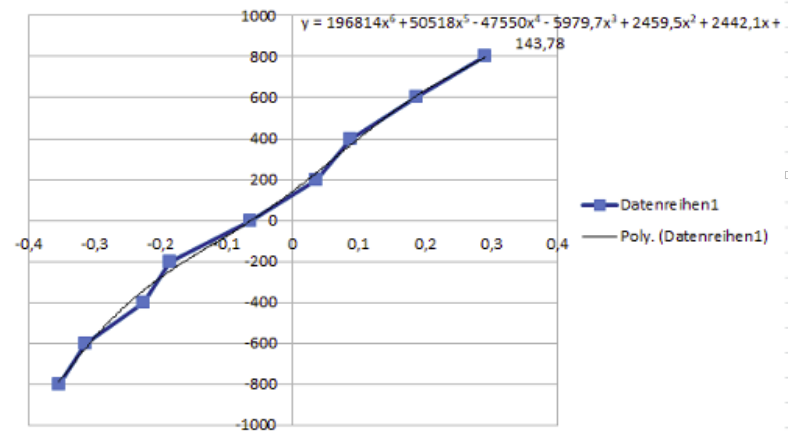
\includegraphics[width=0.7\linewidth]{pics/steering_profile}
	\caption{Lenkwinkelmodell}
	\label{fig:steering_profile}
\end{figure}
\subsection{PD Regler}
\label{subsec:02PDregler}

Ein einfacher Ansatz f\"ur den Rundkurs ohne Hindernisse ist die Abstandregelung mit Hilfe der Ultraschallsensoren und einem PID Regler. Die zu regelnde Gr\"o\ss{}e ist der Abstand zur Wand, als Stellgr\"o\ss{}e dient der Lenkwinkel. Dazu kann entweder die Stellgr\"o\ss{}e f\"ur den Lenkwinkel geregelt werden oder der Lenkwinkel selbst und dann auf die Stellgr\"o\ss{}e mit dem Lenkwinkelmodell umgerechnet werden. Die Reglerauslegung ist sowohl per Simulation in Simulink als auch experimentell durchgef\"uhrt worden. \\
Die Simulation beruht auf dem Ackermann-Modell, einem Einspurmodell f\"ur Fahrzeuge. Es lautet

\begin{align} 
	\dot{\varphi}_\text{K} &= \frac{v}{l}\cdot\tan\varphi_\text{L}\\
	\dot{y} &= v \cdot \sin \varphi_\text{K}+v\cdot\frac{l_\text{H}}{l}\cdot\cos\varphi_\text{K}\cdot\tan\varphi_\text{L}.
	\intertext{Durch Linearisierung erh\"alt man}
	\dot{\varphi}_\text{K} &= \frac{v}{l}\cdot\varphi_\text{L}\\
	\dot{y} &= v\cdot\varphi_\text{K}+v\cdot\frac{l_\text{H}}{l}\cdot\varphi_\text{L}.
\end{align}
Dabei ist $\varphi_\text{K}$ der Kurswinkel, $\varphi_\text{L}$ der Lenkwinkel, $v$ die Geschwindigkeit des Fahrzeugs, $l$ der Achsabstand, $l_\text{H}$ der Abstand von der Hinterachse zu einem Referenzpunkt und $y$ der Abstand zur Wand. Mit beiden Systemen wurde in Simulink eine PD-Reglerauslegung durchgef\"uhrt. Es wurden diskrete Systeme betrachtet (vergleiche Abbildung \ref{fig:regelkreis}), die Geschwindigkeit war $\SI[per-mode=fraction]{0.5}{\meter\per\second}$. Der simulierte Verlauf der Sprungantwort ist in Abbildung \ref{fig:SprungantwortSimulink} dargestellt, der Stellgr\"o\ss{}enverlauf in Abbildung \ref{fig:StellgroesseSimulink}.

\begin{figure}[h]
	\centering
	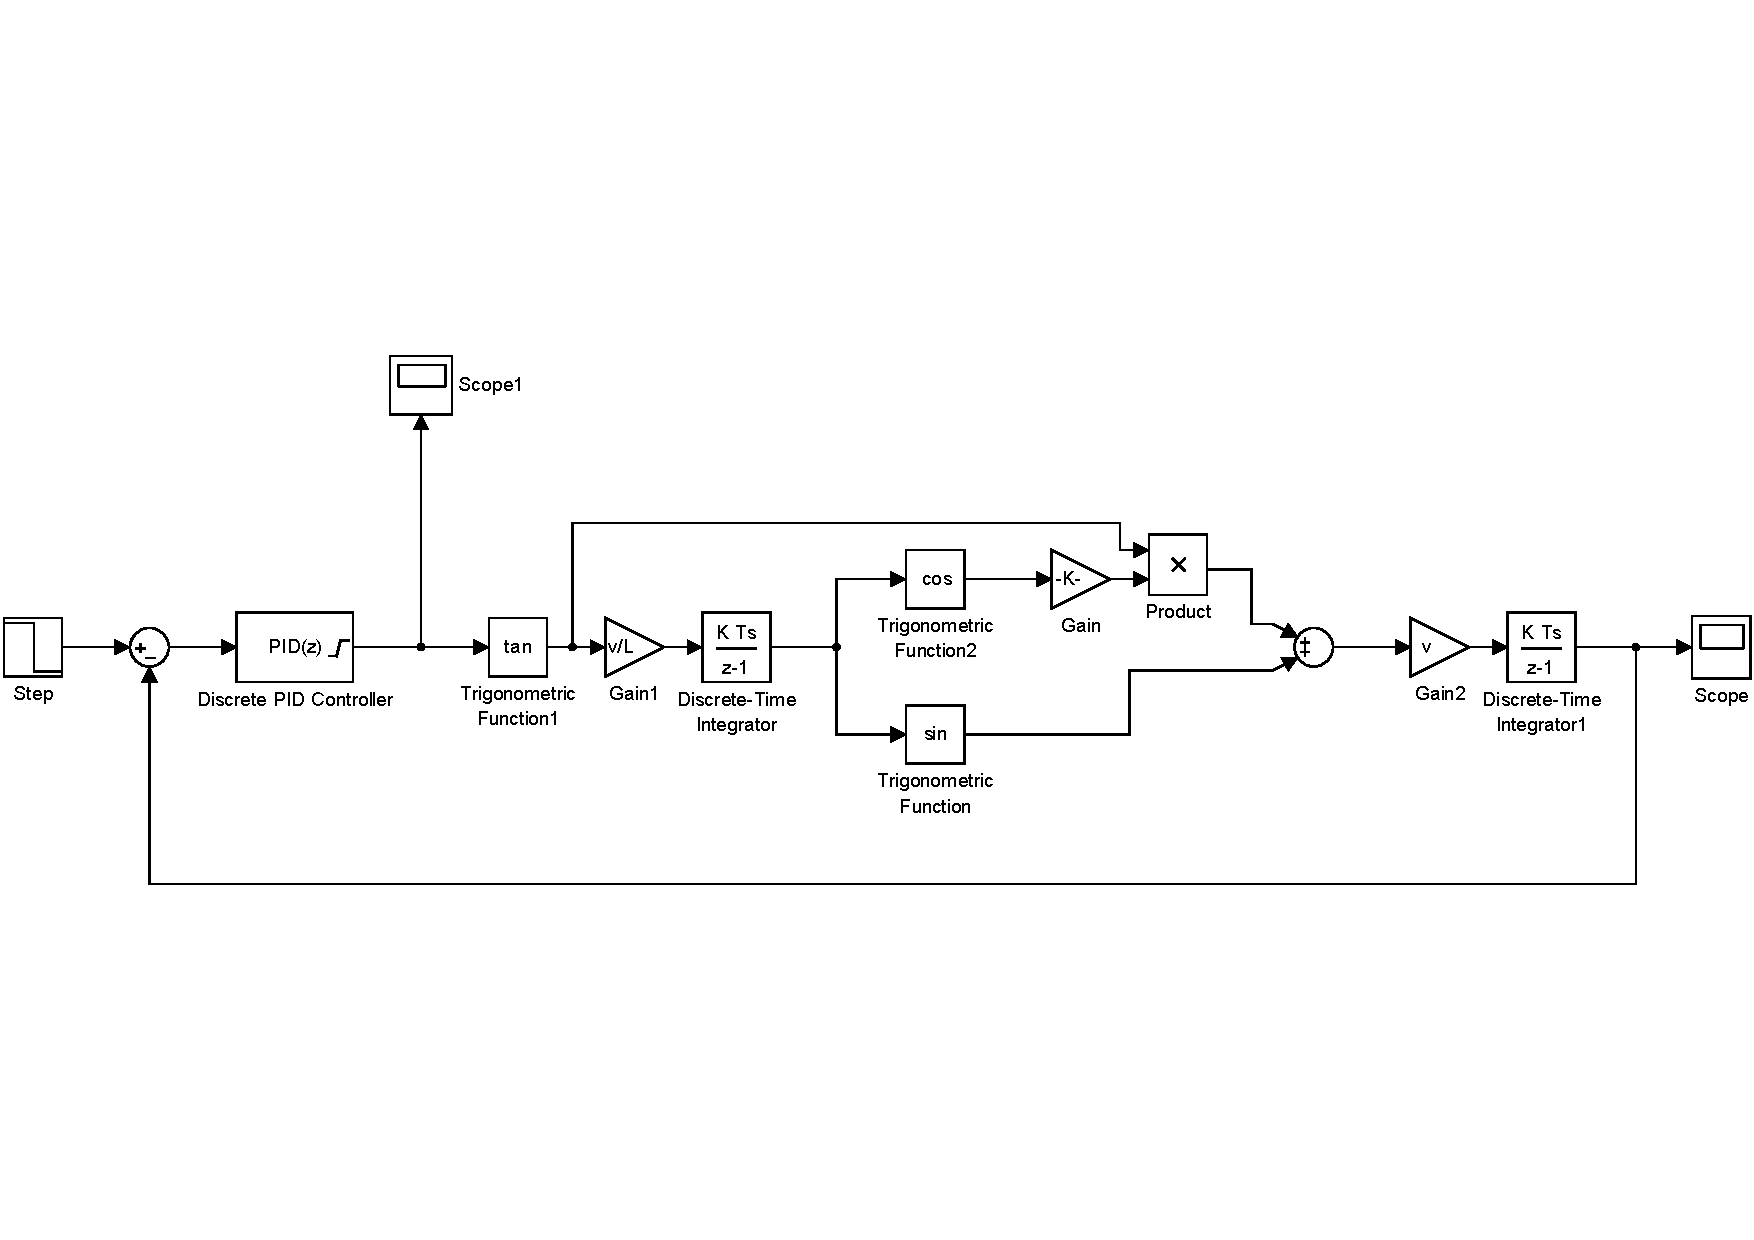
\includegraphics[width=0.9\linewidth,trim=0cm 6cm 0cm 6cm, clip]{pics/system.pdf}
	\caption{Diskreter Regelkreis mit nicht linearisieren Ackermann-Modell.}
	\label{fig:regelkreis}
\end{figure}
\begin{figure}
	\centering
	\subfigure[Sprungantwort]{
			\begin{tikzpicture}
			\begin{axis}[xlabel = Zeit in \si{\second},ylabel=Regelgr\"o\ss{}e in \si{\meter},xmin=0,xmax=9,ymin=0.2, ymax=0.9, axis x line=bottom, axis y line=left,grid,width=7cm,height=5cm]
			\addplot[mark=none,very thick] table [col sep=semicolon] {pics/sprungantwortSimulink.csv};
			\end{axis}
			\label{fig:SprungantwortSimulink}
			\end{tikzpicture}}
	\subfigure[Stellgr\"o\ss{}e]{
			\begin{tikzpicture}
			\begin{axis}[xlabel = Zeit in \si{\second},ylabel=Stellgr\"o\ss{}e in \si{\meter \per \second},xmin=0,xmax=9,ymin=-0.4, ymax=0.4, axis x line=bottom, axis y line	=left,grid,width=7cm,height=5cm]
			\addplot[mark=none,very thick] table [col sep=semicolon] {pics/stellgroesseSimulink.csv};
			\end{axis}
			\label{fig:StellgroesseSimulink}
			\end{tikzpicture}}
	\caption{Simulierte Verl\"aufe des Systems mit $K_\text{p}=10$ und $K_\text{d}=3$.}
	\label{fig:Simulink}
\end{figure}

Mit den gefundenen Parametern konnten keine guten Ergebnisse erzielt werden, der Fahrzeug hat den gew\"unschten Abstand zur Wand nicht eingehalten und ist stark geschwungen. Das ist auf die Ann\"aherung \"uber das Ackermann-Modell und den betrachteten Abstand zu Wand zur\"uckzuf\"uhren. Angenommen wird der Abstand senkrecht zur Wand, der in Wirklichkeit vom Fahrzeug gemessene ist bei schr\"agem Stand jedoch gr\"o\ss{}er. Die Parameter wurden manuell modifiziert und ein zufriedenstellendes Ergebnis erzielt (vergleiche Tabelle \ref{tab:PD}).

\begin{table}[h]
	\centering
	\begin{tabular}{rcc}
		 & $K_\text{p}$ & $K_\text{d}$ \\ 
		Simulink & 10 & 3 \\ 
		Experimentell & 0.48 & 1.5
	\end{tabular}
	\caption{Werte f\"ur PD Regler aus Simulation und experimenteller Bestimmung.}
	\label{tab:PD}
\end{table}

Da die Ergebnisse nicht zufriedenstellend und die L\"osung f\"ur den Rundkurs mit Hindernis nicht praktikabel ist, wurde dieser Ansatz verworfen und am Navigation Stack gearbeitet.

\subsection{Lokalisierung}
\label{subsec:02lokalisierung}

Die Trajektorienplanung des Roboters erfolgt anhand seiner Umgebungskarte, die mit den Sensordaten regelm"a"sig aktualisiert wird. Damit eine gute Trajektorie berechnet werden kann, muss das Fahrzeug in der Lage sein, sich zuverl"assig in der Karte zu lokalisieren. Dies erfordert unter anderem eine verl"assliche Odometrie, die im Abschnitt \ref{subsec:02odom} vorgestellt wird. Um die Position des Fahrzeugs in der Karte genauer zu sch"atzen, wird au"serdem das AMCL-Paket verwendet, wie im Abschnitt \ref{subsec:02amcl} beschrieben ist.

\subsubsection{Odometrie}
\label{subsec:02odom}
Auf dem Fahrzeug befinden sich ein Drei-Achs-Geschwindigkeitssensor und ein Drei-Achs-Gyroskop, welche etwa alle $\SI{0.5}{\milli\second}$ neue Werte zur Verf\"ugung stellen. Diese werden im vorhandenen Odometriepaket \texttt{pses\_odometrie} genutzt um eine Position und die Ausrichtung des Fahrzeugs anzugeben. Durch das Rauschen der Sensoren unterscheidet sich die tats\"achliche Position  nach einiger Zeit von der angegebenen Fahrzeugposition. Die IMU (inertial measurement unit) wird im Odometriepaket zwar zu Beginn kalibriert, dies bedeutet jedoch nur, dass ein festgelegter, im Stand gemittelter Rauschwert ber\"ucksichtigt und von den IMU Daten subtrahiert wird.\\
Die Verwendung eines Extended Kalmanfilters (EKF) erm\"oglicht die Verwendung verschiedener Sensoren als Eingangsgr\"o{\ss}en f\"ur die Sch\"atzung der Fahrzeugposition und der Ausrichtung. Der EKF berechnet aus dem aktuellen Zustand anhand eines nicht-linearen Zustands\"ubergangsmodells eine Absch\"atzung f\"ur den n\"achsten Fahrzeugzustand. Durch die Verwendung mehrerer Sensoren kann die Genauigkeit und Zuverl\"assigkeit der Sensoren mithilfe einer Gewichtung der Eingangsgr\"o{\ss}en des EKF ber\"ucksichtigt werden.  Die Zustandssch\"atzung wird mit der n\"achsten Messung verglichen und die Gewichtung der Sensoren dynamisch angepasst.\\
Wir haben uns f\"ur das \texttt{robot\_localization} Paket entschieden. Dies enth\"alt einen EKF, das es erm\"oglicht die Sensoren modular einzubinden und sensorspezifisch zu entscheiden, welche Daten weiterverarbeitet werden sollen.
Das Paket kann vier verschiedene Topic-Typen verarbeiten:
\begin{itemize}
	\item \texttt{nav\_msgs/Odometry} enh\"alt Positions- und Ausrichtungsdaten
	\item \texttt{geometry\_msgs/PoseWithCovarianceStamped} enth\"alt Positionsdaten
	\item \texttt{geometry\_msgs/TwistWithCovarianceStamped} enth\"alt Ausrichtungsdaten
	\item \texttt{sensor\_msgs/IMU} enth\"alt die Rohdaten aus der Inertialen Messeinheit (IMU)
\end{itemize}
Um die Sch\"atzung zu vereinfachen wird angenommen, dass sich das Fahrzeug nur im zweidimensionalen Raum befindet und nur in X-Richtung fortbewegen kann. Z-Koordinate, Roll- und Pitch Winkel sind daher konstant Null. Die Beschleunigung in Y-Richtung wird als Eingangsr\"o{\ss}e vernachl\"assigt. \\
Das \texttt{robot\_localization} Paket erm\"oglicht es, die Kamera in Verbindung mit \hyphenation{AMCL} AMCL, dem Hall-Sensor und der IMU als Eingangsgr\"o{\ss}en f\"ur das EKF zu verwenden. Aus Zeitgr\"unden haben wir das EKF nicht fertig eingestellt, stattdessen verwenden wir f\"ur die Lokalisierung die Odometriedaten in Verbindung mit AMCL, wie im Abschnitt \ref{subsec:02amcl} beschrieben wird. Dies liefert uns eine ausreichend genaue Fahrzeugposition und Ausrichtung.

\subsubsection{AMCL}
\label{subsec:02amcl}

Zur Lokalisierung des Autos wird das von ROS bereitgestellte AMCL-Paket verwendet. Dieses Paket implementiert den probabilistischen \emph{Adaptive Monte Carlo Localization} - Algorithmus und erm"oglicht dadurch die 2D-Lokalisierung von Robotern in einer vorgegebenen Karte. Die Daten aus dem Laserscan werden auf die Karte projiziert, woraus die wahrscheinlichsten Position und Ausrichtung des Fahrzeugs bestimmt werden.\\
Zu diesem Zweck ben"otigt es mehrere Informationen, n"amlich : 
\begin{itemize}
\item einen Laserscan, der aus den Kameradaten erzeugt wird 
\item die Transformationen zwischen den verschiedenen Koordinatensystemen des Roboters
\item die initiale Position des Roboters, die in unserem Fall manuell durch Rviz "ubergeben wird
\item die Karte, in der der Roboter sich orten soll
\end{itemize}

Diese Topics werden gleicherma"sen vom Navigation Stack ben"otigt und werden deswegen im entsprechenden Kapitel (siehe \ref{subsec:02implementierung}) n"aher beschrieben.\\
Allerdings ist darauf hinzuweisen, dass AMCL eine explizite Transformation vom Laserscan-Frame (hier, \texttt{base\_laser}) zum Odometrie-Frame (hier, \texttt{odom}) erfordert.\\
Das AMCL-Paket stellt ebenso eine ganze Menge von einstellbaren Optimierungsparametern bereit. Es ist zum Beispiel m"oglich das Odometriemodell (\texttt{omni} bzw. \texttt{diff} f"ur Roboter mit omnidirektionalem bzw. Differentialantrieb) auszuw"ahlen, sowie die entsprechenden Parametern einzustellen. Aus zeitlichen Gr"unden wurde jedoch eine im Navigation Stack bereits vorhandene Launchdatei f"ur differentialgetriebene Fahrzeuge (\texttt{amcl\_diff.launch}) verwendet.
\subsection{SLAM}
\label{subsec:02slam}

Die Abk"urzung SLAM steht f"ur \emph{Simultaneous Localization And Mapping} und besteht f"ur einen Roboter darin, gleichzeitig eine Karte seiner Umgebung zu erstellen bzw. zu verbessern und sich darin zu lokalisieren. In ROS stehen mehrere Pakete zur Verf"ugung, welche SLAM implementieren, die bekanntesten sind \texttt{gmapping} und \texttt{hector\_slam}. Letzteres hat die Eigenschaft, dass es keine Odometriedaten ben"otigt und nur anhand des Laserscans die Karte erstellt.\\
Um eine realistische Karte aufzubauen sind mehrere Aspekte zu beachten. Das Fahrzeug sollte langsam und m"oglichst geradeaus (ohne Schwingungen) fahren, um zu vermeiden, dass Fehldetektionen in die Karte eingebaut werden. Die Verwendung der vom Fachgebiet bereitgestellten Pakete \texttt{pses\_dashboard} und \texttt{CarControl-App} k\"onnen zur Steuerung des Fahrzeugs genutzt werden. Falls \texttt{gmapping} benutzt wird, h\"angt die Qualit"at der Karte und Lokalisierung ebenso von der Genauigkeit der Odometriedaten ab.\\
Das \texttt{hector\_slam}-Paket wurde zum Aufbau einer Karte des Fachgebiets verwendet. Da die Qualit"at der Karte jedoch nicht zufriedenstellend war, wurde die von den Tutoren vorgelegte Karte verwendet.
\subsection{Implementierung und Umsetzung}
\label{subsec:02implementierung}

\subsubsection{Navigation Stack}
\label{subsubsec:02navigatinStack}

\paragraph{Costmap}
\paragraph{Globaler Planer}
\paragraph{Lokaler Planer}
\paragraph{TF}
\subsubsection{psesTrajectory TODO} %TODO
\label{subsec:02psesTrajectory}
\paragraph{Modelle}

\paragraph{Zielsetzung}

\subsection{Ergebnisse und Probleme}
\label{subsec:02ergebnisse}
Wie im Kapitel \ref{subsec:02odom} bereits erw\"ahnt, wurde das Extended Kalmanfilter nicht fertig eingestellt. Das implementierte EKF benutzt die IMU-Daten und die Geschwindigkeit, welche mit Hilfe des Hall-Sensors berechnet wird. Obwohl die $y$-Geschwindigkeit des Fahrzeugs nicht als Eingabegr\"o{\ss}e f\"ur das EKF verwendet wird und nur die Steuerung der Geschwindigkeit in $x$-Richtung und des Yaw Winkels zugelassen sind, bewegt sich das Auto in den gefilterten Odometriedaten des EKF seitw\"arts. Das Einstellen der maximalen Be- und Entschleunigungswerte des Fahrzeugs hat zwar zur Verbesserung der Absch\"atzung beigetragen, das Problem der seitlichen Bewegung jedoch nicht behoben.
